\documentclass[10pt]{beamer}
\usepackage[style=verbose,backend=biber]{biblatex}
\usepackage{amsmath}
\usepackage{amssymb}
\usepackage{bookmark}
\usepackage{hyperref}
\usetheme{Madrid}
\addbibresource{main.bib}
\newcommand{\citecomma}{\({}^{{}_{,}}\)}
\renewcommand{\footnotesize}{\tiny}

\title[E2E DL of Opt Heuristics]{End-to-End Deep Learning of Optimization Heuristics}
\subtitle{Presented as a part of \\
CS3423 - Compilers II}
\author[Chris Cummins \textit{et al}]{\textbf{Chris Cummins, Pavlos Petoumenos, Zheng Wang, Hugh Leather}\\
\vspace{10mm}
Vishwak Srinivasan\\
\texttt{CS15BTECH11043}}

\begin{document}
\begin{frame}
\titlepage
\end{frame}

\begin{frame}{Decision making with \emph{heuristics}}
\begin{itemize}
\item<1->{Choice of Optimization techniques is an important decision made during the course of compilation
          \begin{itemize}
          \item<2->{Should a optimization be applied?}
          \item<3->{How should a particular optimization be applied?}
          \end{itemize}}
\item<4->{Such decisions are made by a compilers by means of \emph{heuristics}
          \begin{itemize}
          \item<5->{These heuristics affect the performance of the program}
          \end{itemize}}
\end{itemize}
\end{frame}

\begin{frame}{What these \emph{heuristics}?}
\begin{itemize}
\item{There are two kinds of heuristics (broadly)
      \begin{itemize}
      \item<1->{Hand-written heuristics \textit{(Briggs Heuristic for Register Allocation\footfullcite{Briggs:1989:CHR:73141.74843}, for instance)}}
      \item<2->{Predictive modelling based heuristics}
      \end{itemize}}
\item<3->{This paper focuses on predictive modelling using Deep Learning techniques}
\end{itemize}
\end{frame}

\begin{frame}{Design Decisions - Pipeline of an earlier predictive model}
Studies prior to this work suggested the usage of a pipelined model as shown below:
\begin{figure}[H]
\centering
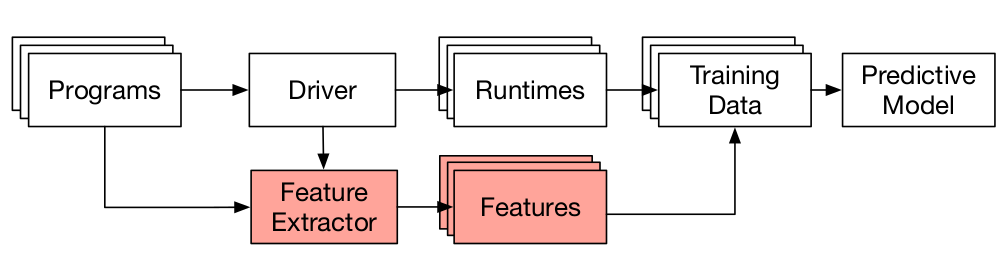
\includegraphics[width=0.7\textwidth]{old-pipeline.png}
\end{figure}

\uncover<1->{Note the feature extraction phase, which is done \underline{manually}}
\(\newline\)

\uncover<2->{Some disadvantages include: }
\begin{itemize}
\item<3->{Failure to identify an important feature has a negative effect on the resulting heuristic}
\item<4->{This could possibly take a lot of time and effort}
\end{itemize}
\end{frame}
\begin{frame}{Design Decisions - Pipeline of the proposed predictive model}
The proposed predictive model follows a pipelined model as shown below:
\begin{figure}[H]
\centering
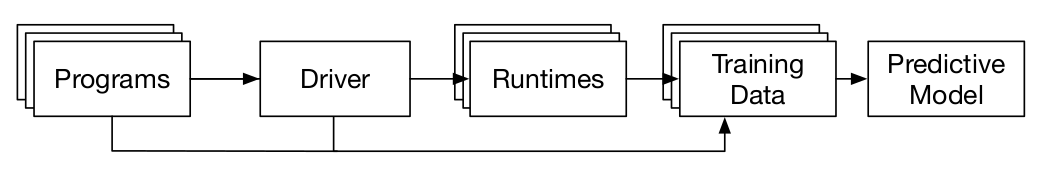
\includegraphics[width=0.7\textwidth]{new-pipeline.png}
\end{figure}

\uncover<1->{Note that the feature extraction phase is bypassed and the methodology learns directly from code}
\(\newline\)

\uncover<2->{Advantages of this methodology are:}
\begin{itemize}
\item<3->{The models find out rationally what the essential features are}
\item<4->{Human error could be removed}
\end{itemize}
\end{frame}

\begin{frame}{Novelty of the paper}
\begin{itemize}
\item<1->{Although techniques for automatic feature generation from the compiler's IR have been proposed\footfullcite{Namolaru:2010:PAS:1878921.1878951}\citecomma\footfullcite{Leather:2014:AFG:2591460.2536688}, these do not solve the problem of feature extraction in a practical way}
\item<2->{Using ideas from deep learning and language modelling, the proposed methodology hinges on the fact that representations of the raw code would behave as features extracted}
\item<3->{Instead of manual feature extraction to get training data, program code is directly used as training data}
\item<4->{This training data is then fed through a series of neural networks which learn correlation and relative importance between features and performance}
\item<5->{Clearly, the proposed methodology eliminate the requirement of static features, effectively by combining feature and heuristic selection into one problem}
\item<6->{Encorporates \textit{transfer learning}, which results in high-quality heuristics even when trained on a small number of programs}
\end{itemize}
\end{frame}

\begin{frame}{Contributions of the paper and problems addressed}
Contributions of this paper are:
\begin{itemize}
\item<1->{Methodology for building compiler heuristics}
\item<2->{Tool called \emph{DeepTune}, which combines all the novelties of the presented earlier}
\end{itemize}
\(\newline\)

\uncover<3->{Problems addressed in the paper are:}
\begin{itemize}
\item<3->{Heterogeneous Device Mapping on OpenCL
          \begin{itemize}
          \item<3->{OpenCL is a platform-agnostic framework for heterogeneous parallelism, meaning the same code can be run on multiple devices (CPUs, GPUs, FPGAs) parallely}
          \item<3->{Which devices should the code run on to maximize performance?}
          \end{itemize}}
\item<4->{GPU Thread Coarsening
          \begin{itemize}
          \item<4->{Thread Coarsening is an optimization for parallel programs where the operations of two or more threads are fused together}
          \item<4->{May or may not prove to be beneficial based on what is being executed on different threads}
          \end{itemize}}
\end{itemize}
\end{frame}

\begin{frame}{DeepTune}
\begin{figure}[H]
\centering
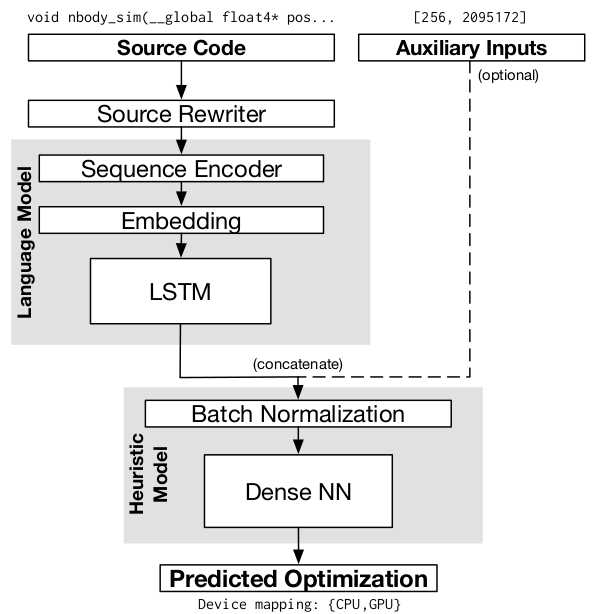
\includegraphics[height=0.6\textwidth]{deeptune.png}
\end{figure}
\end{frame}

\begin{frame}{DeepTune: An Overview}
\begin{itemize}
\item<1->{Primary input is the source code of a program to be optimized, through a series of neural nets}
\item<2->{Directly predicts the optimization that should be applied}
\item<3->{Independent of compiler, platform or optimization problem, which means that you can use a similar design for a different purpose too}
\item<4->{Open Source!!\footnote{\url{https://chriscummins.cc/deeptune}}}
\end{itemize}
\end{frame}

\begin{frame}{DeepTune: Source Rewriter}
\begin{itemize}
\item<1->{First phase}
\item<2->{Canonicalizes the code to a ``standard form", using \emph{source normalizing} techniques\footfullcite{Cummins:2017:SBP:3049832.3049843}
         \begin{itemize}
         \item<2->{These techniques are implemented as an LLVM Pass}
         \item<3->{Rebuilds the input source code using a consistent code style and identifier naming scheme}
         \end{itemize}}
\end{itemize}
\uncover<4->{
\begin{minipage}{0.45\linewidth}
\begin{figure}[H]
\centering
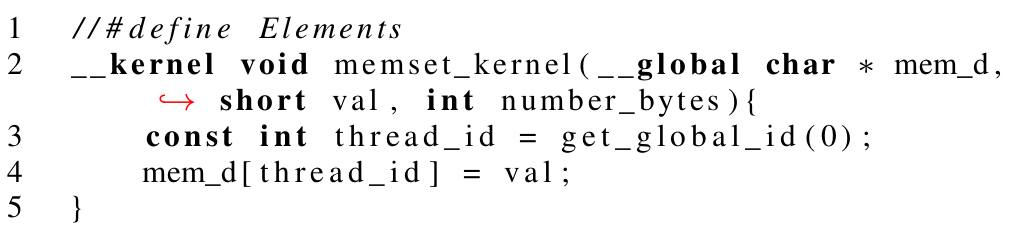
\includegraphics[width=0.95\textwidth]{before-src-rw.png}
\end{figure}
\end{minipage}
\Large\(\Rightarrow\)\hfill
\begin{minipage}{0.45\linewidth}
\begin{figure}[H]
\centering
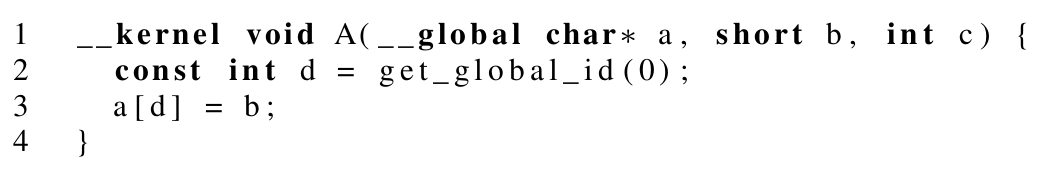
\includegraphics[width=0.95\textwidth]{after-src-rw.png}
\end{figure}
\end{minipage}
}
\end{frame}

\begin{frame}{DeepTune: Sequence Encoder}
\begin{itemize}
\item<1->{First phase on language model}
\item<2->{Encode the now canonicalized source code as a string of integers for interpretation by neural networks
          \begin{itemize}
          \item<3->{Each integer mapping comes from a table of indices contains predetermined vocabulary (characters, tokens)}
          \end{itemize}}
\item<4->{Previous work used a \emph{character-based} vocabulary\footfullcite{Cummins:2017:SBP:3049832.3049843}, and a \emph{token-based} vocabulary\footfullcite{Allamanis:2013:MSC:2487085.2487127}
          \begin{itemize}
          \item<5->{\emph{Character-based} vocabulary leads to long, uninteresting sequences, from which extracting information is hard}
          \item<6->{\emph{Token-based} vocabulary leads to short sequences, but a larger vocabulary itself}
          \end{itemize}}
\item<7->{This work uses a hybrid approach, where tokens are considered directly in the vocabulary, whereas literals and unfrequently used words are encoded at character level}
\end{itemize}
\end{frame}

\begin{frame}{DeepTune: Sequence Encoder}
\begin{minipage}{0.45\linewidth}
\begin{figure}[H]
\centering
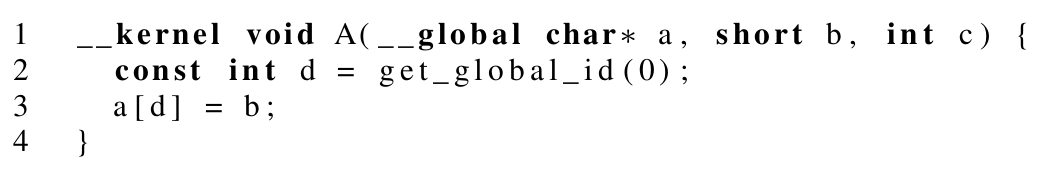
\includegraphics[width=0.95\textwidth]{after-src-rw.png}
\end{figure}
\begin{center}
\Large\(\Downarrow\)
\end{center}
\begin{figure}[H]
\centering
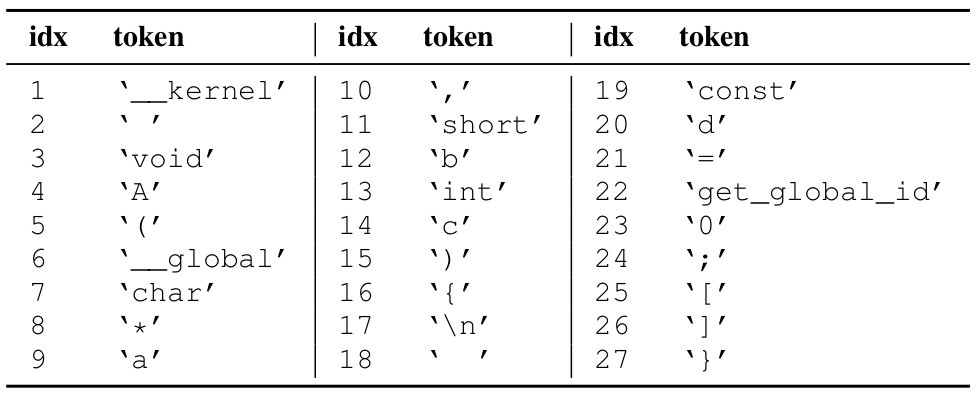
\includegraphics[width=0.95\textwidth]{vocab.png}
\end{figure}
\end{minipage}
\Large\(\Rightarrow\)\hfill
\begin{minipage}{0.45\linewidth}
\begin{figure}[H]
\centering
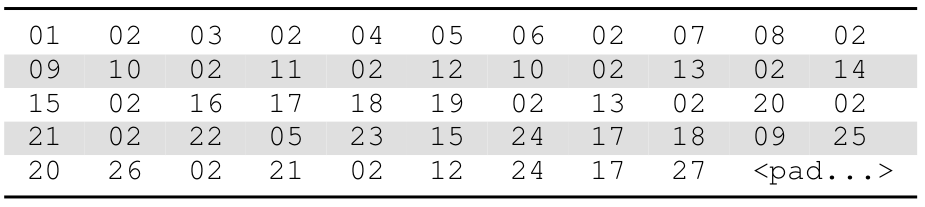
\includegraphics[width=0.95\textwidth]{seq-enc.png}
\end{figure}
\end{minipage}
\end{frame}

\begin{frame}{DeepTune: Embedding}
\begin{itemize}
\item<1->{Second phase of language model}
\item<2->{A direct encoding could lead to static, but randomly assigned integers to tokens
          \begin{itemize}
          \item<3->{This could lead to a situation where the language model will not be able to infer relationships based on these mappings}
          \end{itemize}}
\item<4->{To help avoid this issue, the paper proposes an embedding of tokens, which effectively will map tokens from a sparse, integer encoded vocabulary into a lower dimensional space
          \begin{itemize}
          \item<5->{This enables related tokens like \texttt{int} and \texttt{float} to be mapped to nearby points}
          \end{itemize}}
\item<6->{Mathematically, given a vocabulary size of \(V\) and an embedding dimensionality \(D\), \(\mathbf{W_{E}} \in \mathbb{R}^{V \times D}\) is learnt during training. Tokens, which are \(\mathbf{t} \in \mathbb{N}^{L}\) are now mapped to \(\mathbf{T} \in \mathbb{R}^{L \times D}\)}
\end{itemize}
\end{frame}

\begin{frame}{DeepTune: Sequence Characterization using LSTMs}
\begin{itemize}
\item<1->{Final phase of language model}
\item<2->{LSTM\footfullcite{lstm} invented as a modification to RNNs to reduce the effect of vanishing gradients}
\item<3->{These have been shown to be extremely powerful in language modelling, and effective in learning complex relationships across long sequences\footfullcite{lstm-benefits}}
\item<4->{This paper uses a two layer LSTM to characterize a given sequence of embedding vectors, and returns a single output vector, characterizing the entire sequence}
\end{itemize}
\end{frame}

\begin{frame}{DeepTune: Auxilary Inputs}
\begin{itemize}
\item<1->{Auxiliary inputs are used to augment the source code input}
\item<2->{Can be thought of increasing the flexibility of \emph{DeepTune}
          \begin{itemize}
          \item<2->{For example, this can be used to support applications where the optimization heuristic depends on dynamic values, which cannot be statically determined from the source code}
          \end{itemize}}
\end{itemize}
\end{frame}

\begin{frame}{DeepTune: The Heuristic Model and training the model}
\begin{itemize}
\item<1->{After obtaining the learned representations of the source code and auxiliary inputs (if any), we pass them through a fully connected neural network to make predictions about the optimization to be used}
\item<2->{\emph{DeepTune} uses batch normalization\footfullcite{batchnorm} where the inputs are transformed based on the below mapping:
          \vspace{-4mm}\[x'_{i} = \gamma_{i}\displaystyle\frac{x_{i} - \mathbb{E}(x_{i})}{\sqrt{\mathrm{Var}[x_{i}]}} + \beta_{i}\]}
\item<3->{\texttt{ReLU} activation functions\footfullcite{Nair:2010:RLU:3104322.3104425} are placed between layers and a \texttt{sigmoid} activation function at the last layer to provide output in the range \((0, 1)\)}
\item<4->{Uses a cross entropy loss function to train. Mathematically, parameters learned are given by
\vspace{-5mm}\[\Theta^{*} = \mathrm{arg}\min_{\Theta} \displaystyle \frac{1}{n}\sum_{i=1}^{n}\mathcal{L}(X_{i}, \Theta)\]}
\vspace{-5mm}
\item<5->{The optimization problem posed above is solved using Adam\footfullcite{adam-iclr}, with batches
          \begin{itemize}
          \item<6->{All the inputs in a batch are supposed to be of the same size, hence padding is done}
          \end{itemize}}
\end{itemize}
\end{frame}

\begin{frame}{Experimental Results: OpenCL Heterogeneous Mapping}
\begin{itemize}
\item<1->{Previous work by Grewe \textit{et al}\footfullcite{grewe} consider a decision tree based approach based on a set of expert chosen features
         \begin{itemize}
         \item<2->{Features are both static and dynamic: static features are extracted from LLVM and dynamic features are extracted from OpenCL runtime}
         \end{itemize}}
\end{itemize}
\uncover<3->{
\begin{minipage}{0.45\linewidth}
\begin{figure}[H]
\centering
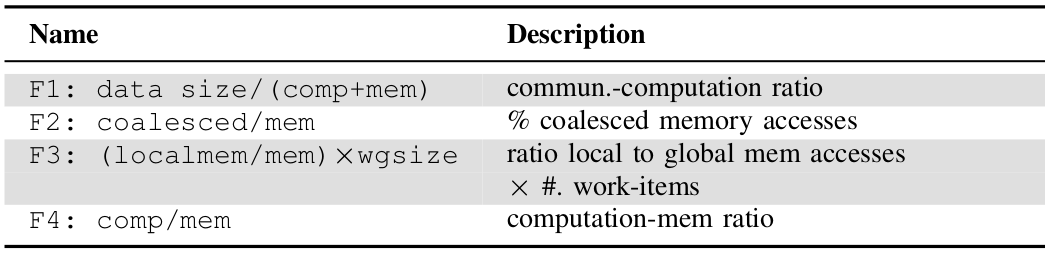
\includegraphics[width=0.95\textwidth]{hmap-grewe.png}
\end{figure}
\end{minipage}
\hfill
\begin{minipage}{0.45\linewidth}
\begin{figure}[H]
\centering
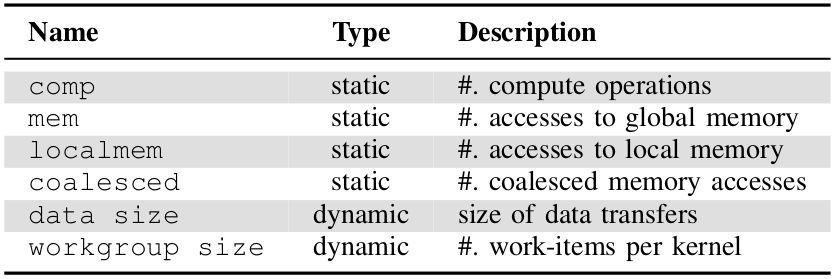
\includegraphics[width=0.95\textwidth]{hmap-grewe-values.png}
\end{figure}
\end{minipage}}
\end{frame}

\begin{frame}{Experimental Results: OpenCL Heterogeneous Mapping}
\emph{DeepTune} is configured as follows:
\begin{columns}
\begin{column}{0.5\textwidth}
\begin{figure}[H]
\centering
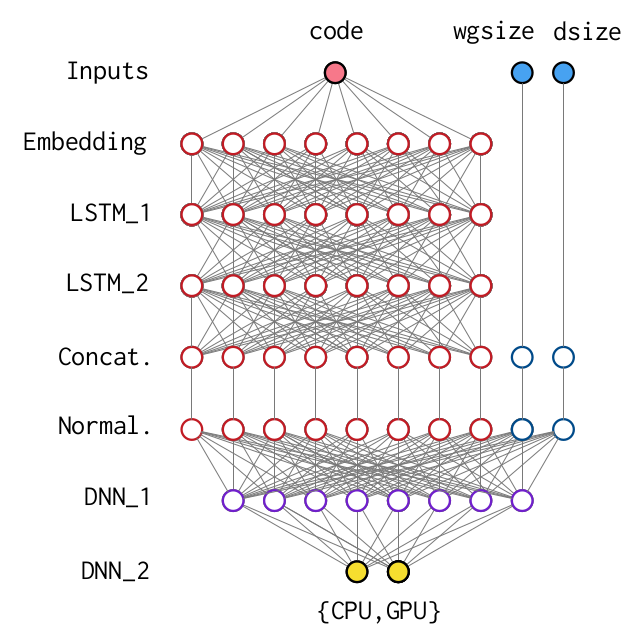
\includegraphics[width=0.95\textwidth]{hmap-deeptune.png}
\end{figure}
\end{column}
\hfill
\begin{column}{0.5\textwidth}
\begin{itemize}
\item{\emph{DeepTune} uses the code as well as two auxiliary inputs: \texttt{wgsize} (work group size) and \texttt{dsize} (data size), dynamically from the OpenCL runtime environment}
\item{Number of parameters and neurons used in \emph{DeepTune}'s configuration is tabulated below:}
\end{itemize}
\begin{tabular}{|l|r|r|}
\hline
\small \textbf{Layer} & \small\#neurons & \small\#parameters \\
\hline
\small \textbf{Embedding} & \small 64 & \small 8256 \\
\small \textbf{LSTM\_1} & \small 64 & \small 33024 \\
\small \textbf{LSTM\_2} & \small 64 & \small 33024 \\
\small \textbf{Batch Norm} & \small 66 & \small 264 \\
\small \textbf{DNN\_1} & \small 32 & \small 2144 \\
\small \textbf{DNN\_2} & \small 2 & \small 66 \\
\hline
\small \textbf{Total} & & \small 76788 \\
\hline
\end{tabular}
\end{column}
\end{columns}
\end{frame}

\begin{frame}{Experimental Results: OpenCL Heterogeneous Mapping}
\begin{itemize}
\item<1->{The paper considers 71 benchmarks and evaluates \emph{DeepTune} on two CPU-GPU setups, tabulated below:}
\end{itemize}
\uncover<1->{
\begin{minipage}{0.4\textwidth}
\begin{figure}[H]
\centering
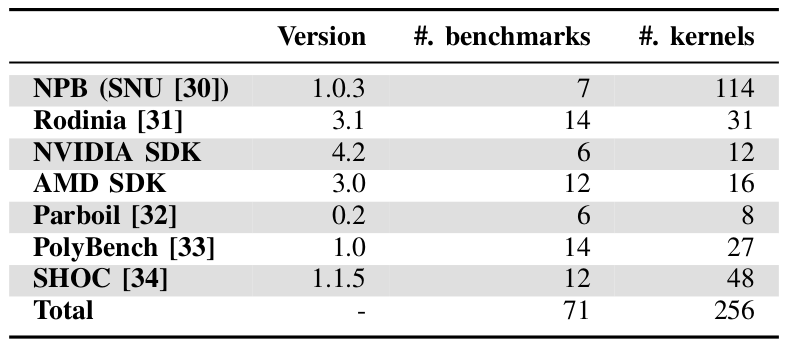
\includegraphics[width=0.95\textwidth]{hmap-bench.png}
\end{figure}
\end{minipage}
\hfill
\begin{minipage}{0.4\textwidth}
\begin{figure}[H]
\centering
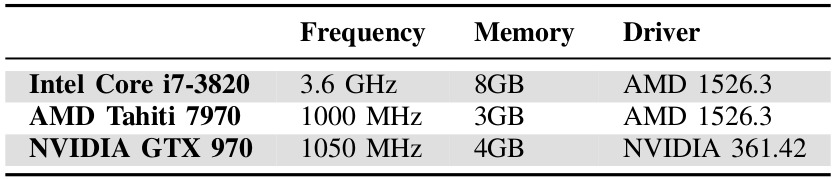
\includegraphics[width=0.95\textwidth]{hmap-device.png}
\end{figure}
\end{minipage}
}
\begin{itemize}
\item<2->{\emph{DeepTune} is compared with the heuristic proposed by Grewe \textit{et al}\footfullcite{grewe} and a static mapping approach, which selects the device the device that gave the best average case performance across all programs}
\item<3->{Below are the accuracy for the optimization heuristics taken into comparison for the two setups}
\end{itemize}
\uncover<3->{
\begin{minipage}{0.4\textwidth}
\begin{figure}[H]
\centering
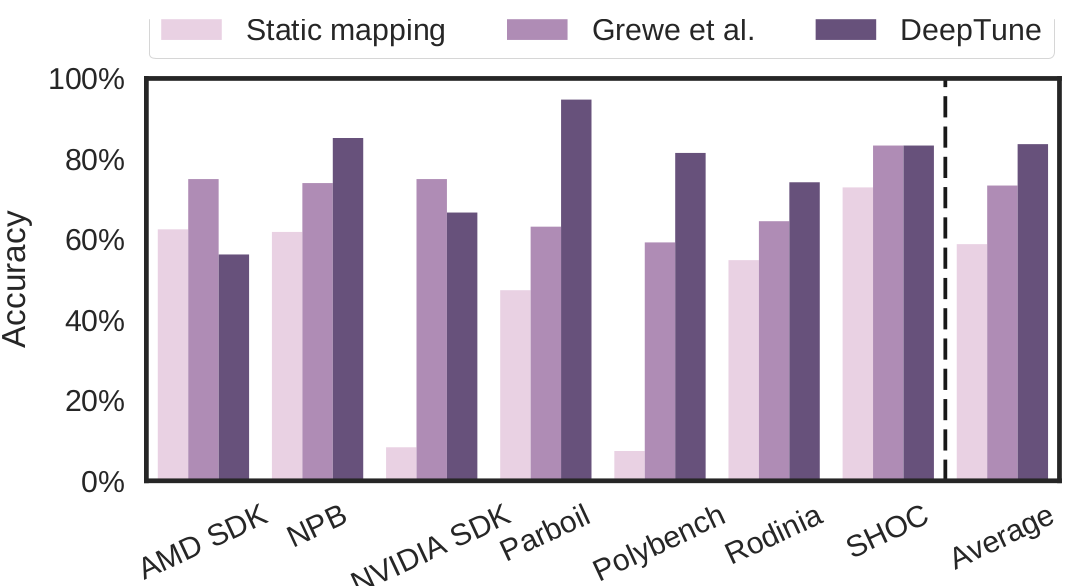
\includegraphics[width=0.95\textwidth]{hmap-acc-1.png}
\end{figure}
\end{minipage}
\hfill
\begin{minipage}{0.4\textwidth}
\begin{figure}[H]
\centering
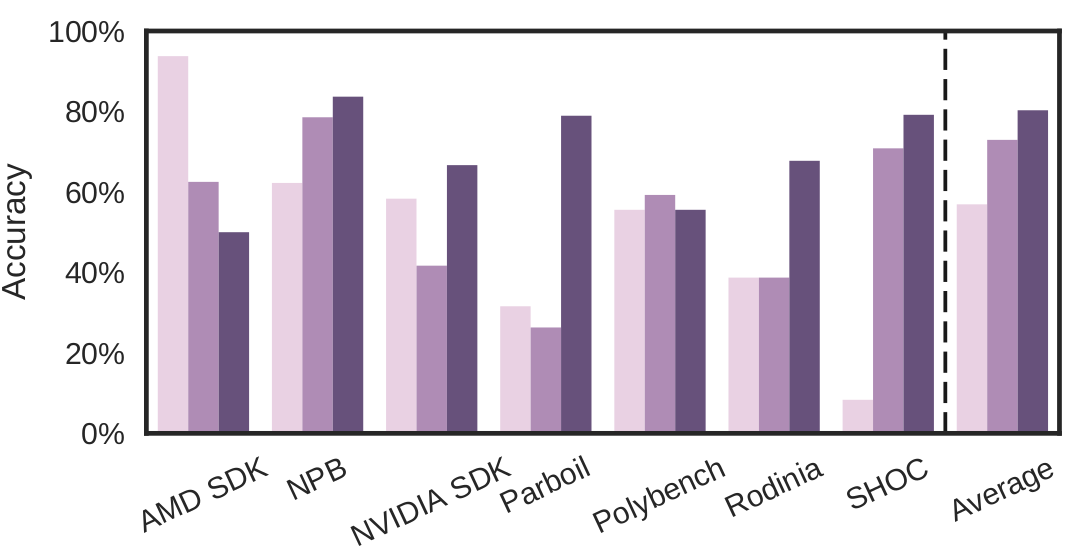
\includegraphics[width=0.95\textwidth]{hmap-acc-2.png}
\end{figure}
\end{minipage}}
\end{frame}

\begin{frame}{Experimental Results: OpenCL Heterogeneous Mapping}
Final Results plotted with Speedup and static mapping and baseline:
\begin{figure}[H]
\centering
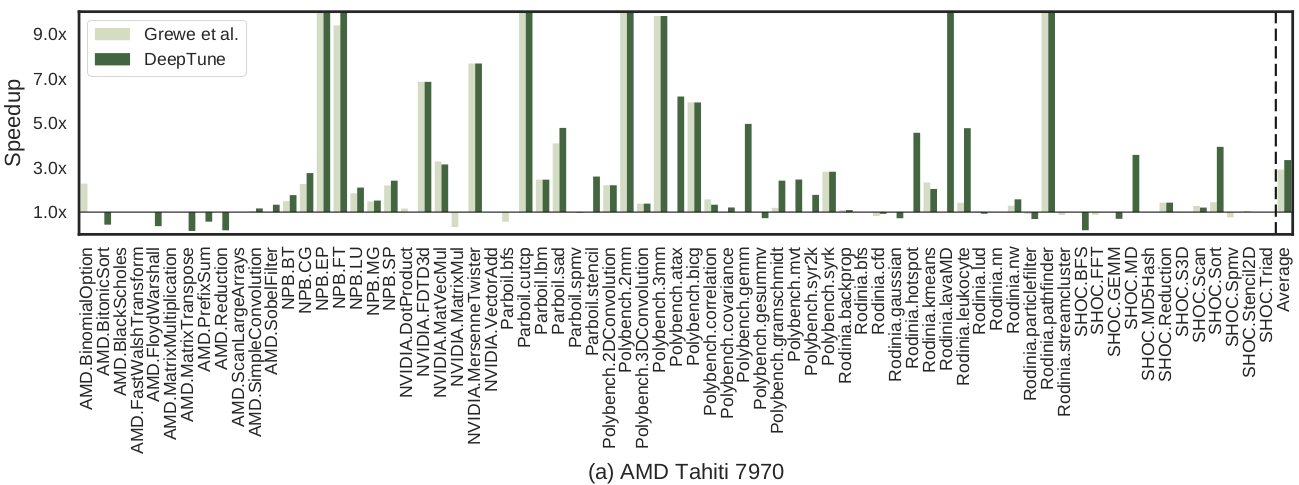
\includegraphics[width=0.8\textwidth]{hmap-res-1.png}
\end{figure}
\vspace{-2mm}
\begin{figure}[H]
\centering
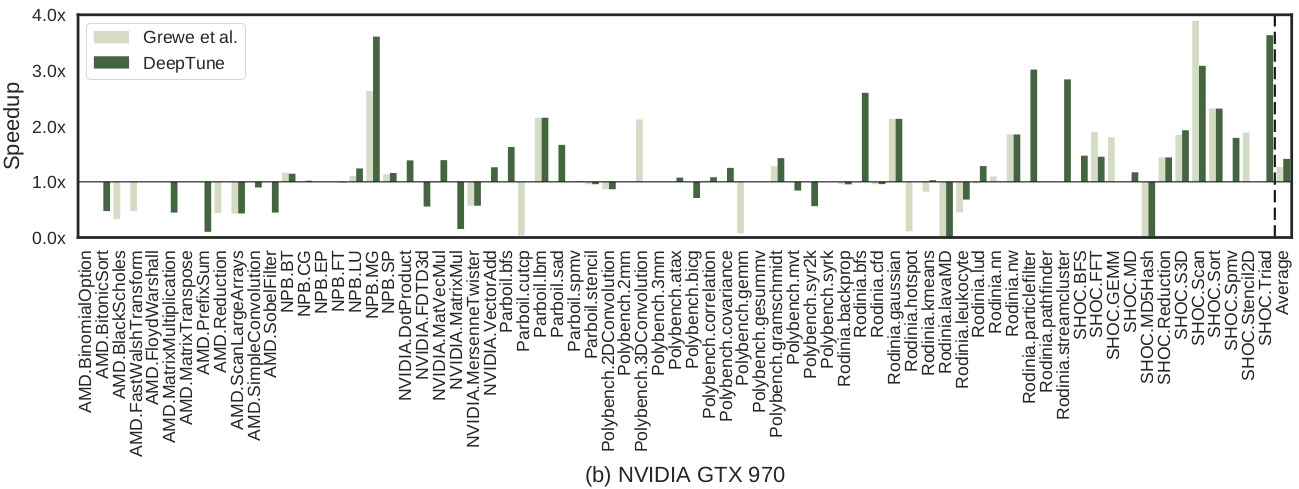
\includegraphics[width=0.8\textwidth]{hmap-res-2.png}
\end{figure}
\end{frame}

\begin{frame}{Experimental Results: OpenCL Thread Coarsening Factor}
\begin{itemize}
\item<1->{Previous work by Magni \textit{et al}\footfullcite{magni} present a predictive model for OpenCL thread coarsening.
          \begin{itemize}
          \item<2->{If a program benefits from coarsening, then coarsen and then check if further coarsening is possible}
          \item<3->{Coarsening is chosen from the set of 6 possible coarsening factors \{1, 2, 4, 8, 16, 32\} based on 17 handpicked features}
          \end{itemize}}
\end{itemize}
\uncover<4->{
\begin{figure}[H]
\centering
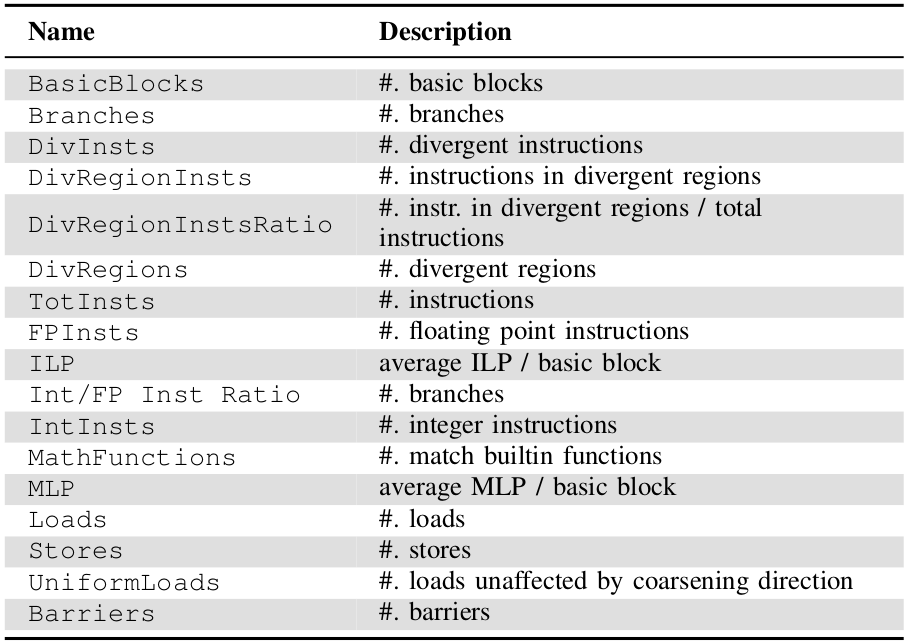
\includegraphics[width=0.6\textwidth]{coarsen-features.png}
\end{figure}
}
\end{frame}

\begin{frame}{Experimental Results: OpenCL Thread Coarsening Factor}
\emph{DeepTune} is configured as follows:
\begin{columns}
\begin{column}{0.5\textwidth}
\begin{figure}[H]
\centering
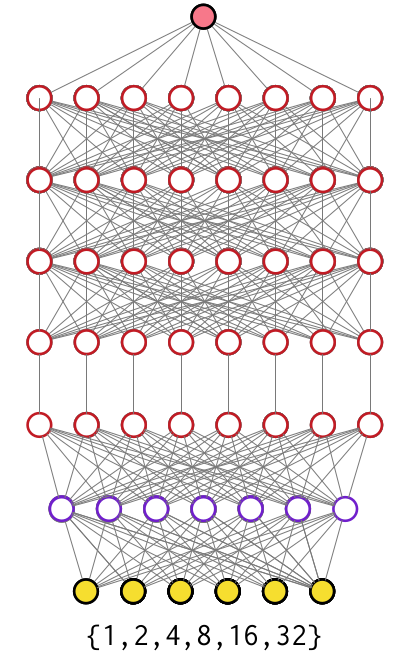
\includegraphics[width=0.7\textwidth]{coarsen-deeptune.png}
\end{figure}
\end{column}
\hfill
\begin{column}{0.5\textwidth}
\begin{itemize}
\item{\emph{DeepTune} uses the code only for predicting coarsening factor}
\item{Number of parameters and neurons used in \emph{DeepTune}'s configuration is tabulated below:}
\end{itemize}
\begin{tabular}{|l|r|r|}
\hline
\small \textbf{Layer} & \small\#neurons & \small\#parameters \\
\hline
\small \textbf{Embedding} & \small 64 & \small 8256 \\
\small \textbf{LSTM\_1} & \small 64 & \small 33024 \\
\small \textbf{LSTM\_2} & \small 64 & \small 33024 \\
\small \textbf{Batch Norm} & \small 64 & \small 256 \\
\small \textbf{DNN\_1} & \small 32 & \small 2080 \\
\small \textbf{DNN\_2} & \small 6 & \small 198 \\
\hline
\small \textbf{Total} & & \small 76838 \\
\hline
\end{tabular}
\end{column}
\end{columns}
\end{frame}

\begin{frame}{Experimental Results: OpenCL Thread Coarsening Factor}
\begin{itemize}
\item<1->{The paper considers 17 benchmarks and 4 experimental platforms where \emph{DeepTune} is tested upon, which are shown below:}
\end{itemize}
\uncover<1->{
\begin{minipage}{0.4\textwidth}
\begin{figure}[H]
\centering
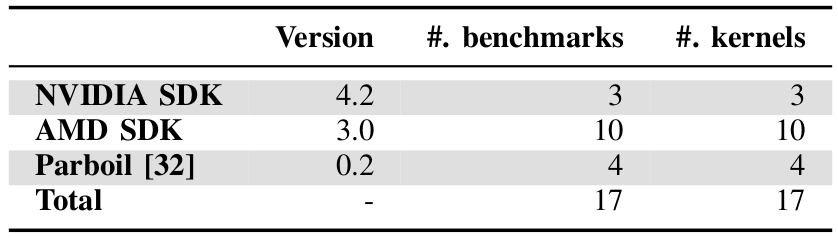
\includegraphics[width=0.95\textwidth]{coarsen-bench.png}
\end{figure}
\end{minipage}
\hfill
\begin{minipage}{0.4\textwidth}
\begin{figure}[H]
\centering
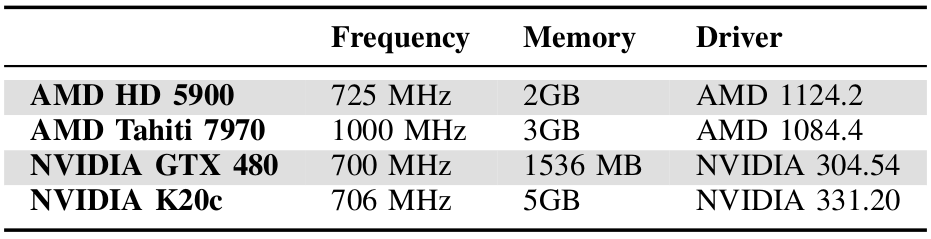
\includegraphics[width=0.95\textwidth]{coarsen-device.png}
\end{figure}
\end{minipage}
}
\begin{itemize}
\item<2->{\emph{DeepTune} is compared with the heuristic proposed by Magni \textit{et al}\footfullcite{magni} and a variant of \emph{DeepTune} with transfer learning called \emph{DeepTune-TL}, since the number of programs are small and thus leads to lower training data
         \begin{itemize}
         \item<3->{This was done by transferring the weights learned for the language modelling part of \emph{DeepTune} for heterogeneous mapping to the language model of \emph{DeepTune} for thread coarsening}
         \end{itemize}}
\end{itemize}
\end{frame}

\begin{frame}{Experimental Results: OpenCL Thread Coarsening Factor}
\begin{minipage}{0.475\linewidth}
\begin{figure}[H]
\centering
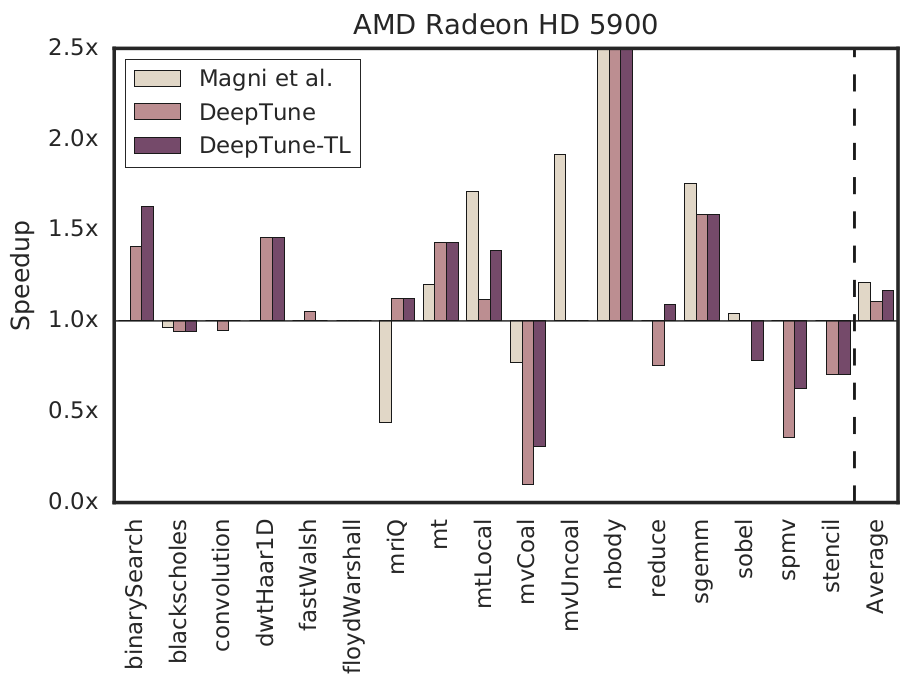
\includegraphics[width=0.9\textwidth]{coarsen-res-1.png}
\end{figure}
\end{minipage}
\hfill
\begin{minipage}{0.475\linewidth}
\begin{figure}[H]
\centering
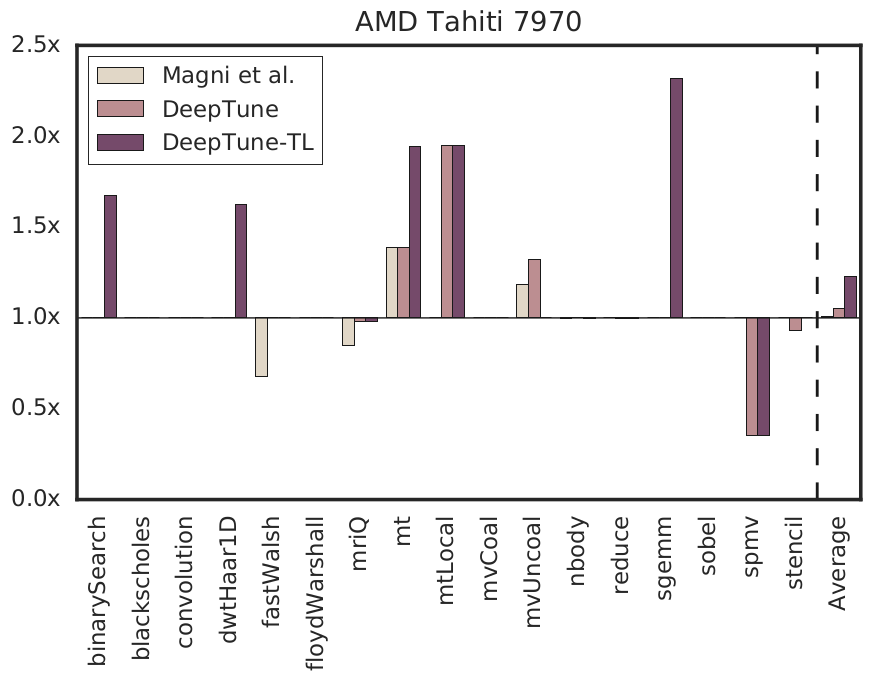
\includegraphics[width=0.9\textwidth]{coarsen-res-2.png}
\end{figure}
\end{minipage}
\vspace{-2mm}
\begin{minipage}{0.475\linewidth}
\begin{figure}[H]
\centering
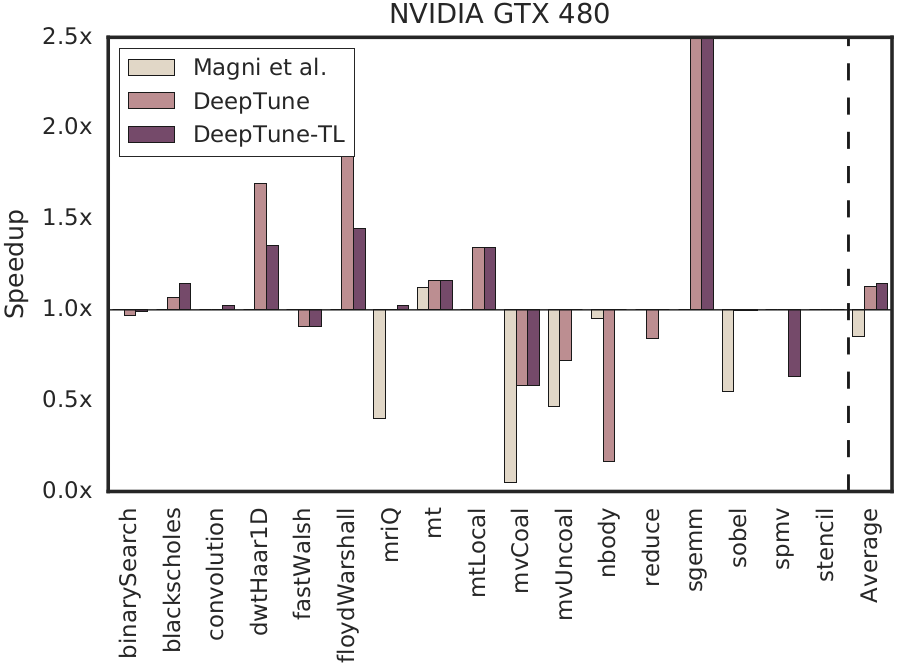
\includegraphics[width=0.9\textwidth]{coarsen-res-3.png}
\end{figure}
\end{minipage}
\hfill
\begin{minipage}{0.475\linewidth}
\begin{figure}[H]
\centering
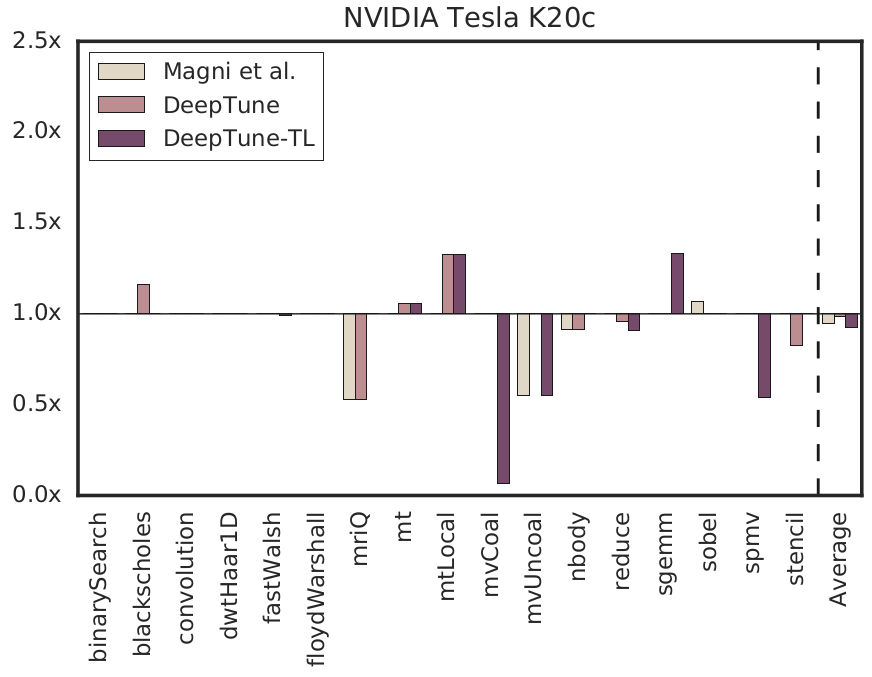
\includegraphics[width=0.9\textwidth]{coarsen-res-4.png}
\end{figure}
\end{minipage}
\end{frame}

\begin{frame}{Internal Activation States of DeepTune}
Taking 267 lines of code from the \texttt{mriQ} kernel code from the Parboil benchmark for OpenCL, the paper shows the internal activation states by means of a heatmap. This program performs 99\% of the maximum performance whereas the state-of-the-art by Magni \textit{et al}\footfullcite{magni} performs upto 54\% of the maximum performance
\vspace{-2mm}
\begin{figure}[H]
\centering
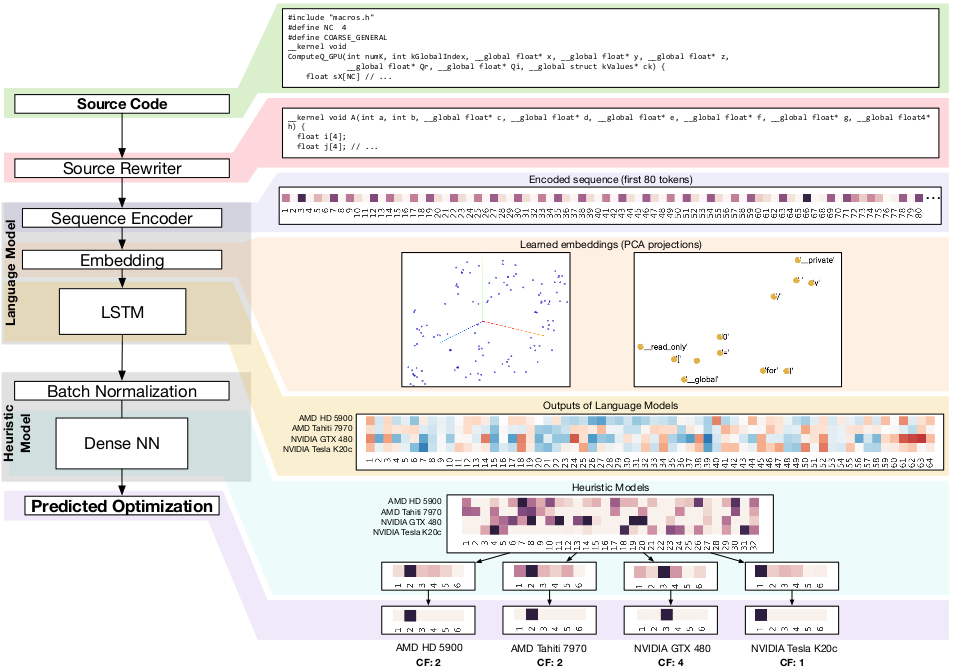
\includegraphics[width=0.65\textwidth]{internal-act.png}
\end{figure}
\end{frame}

\begin{frame}{Prior and Related Work}
\begin{itemize}
\item<1->{Machine Learning techniques have been used to learn from program source code on various tasks}
\item<2->{Mining code conventions\footfullcite{Allamanis:2014:LNC:2635868.2635883} and idioms\footfullcite{Allamanis:2014:MIS:2635868.2635901} and API example code\footfullcite{Gu:2016:DAL:2950290.2950334}, pseudo-code\footfullcite{Oda:2015:LGP:2916135.2916173} and benchmark code generation\footfullcite{Cummins:2017:SBP:3049832.3049843}}
\item<3->{Cavazos \textit{et al}\footfullcite{Cavazos:2006:APM:1176760.1176765} presented a predictive model for software-hardware code design, where they choose best compiler options for a given micro-architecture setting}
\item<4->{Work has also been done where genetic programming and algorithms have been used to search for features\footfullcite{Leather:2009:AFG:1545006.1545059}}
\end{itemize}
\end{frame}

\begin{frame}{Conclusions}
\begin{itemize}
\item<1->{Machine Learning to Optimization prediction requires features first}
\item<2->{Generally done by experts, but is a time and effort consuming process}
\item<3->{\emph{DeepTune} helps bypass this process, and learns features from code directly by relying on powerful language modelling techniques to build representations of source code}
\item<4->{\emph{DeepTune} provides full automation once trained and performs better than the older state-of-the-art models by 14\% and 12\% on heterogeneous mapping and thread coarsening respectively}
\item<5->{Transfer Learning attempted for the first time in predictive modelling, and \emph{DeepTune-TL} has provided a 16\% performance improvement with that also}
\end{itemize}
\end{frame}
\end{document}
